\documentclass[12pt]{article}

\linespread{1.5}
\setlength{\parindent}{0pt}

\usepackage[letterpaper, margin=0.75in]{geometry}
\usepackage{times}  % Times New Roman font
\usepackage{amsmath}
\usepackage{graphicx}
\usepackage{float}
\usepackage{textgreek}
\usepackage[super]{nth}
\usepackage{physics}
\usepackage{titling}
\usepackage{titlesec}
\usepackage{gensymb}

\titleformat*{\section}{\large\bfseries}
\titleformat*{\subsection}{\bfseries}
\titleformat*{\subsubsection}{\itshape}
\makeatletter
\def\@maketitle{%
    \newpage
    \null
    {\@bspretitle \@title \@bsposttitle}
    {\@bspredate \@date \@bspostdate}
    {\@bspreauthor \@author \@bspostauthor}
    \par
    \vskip 1.5em}
\makeatother

% Customize title format
\pretitle{\begin{flushleft}\LARGE\vspace{-1.25cm}}
\posttitle{\end{flushleft}}
\predate{\begin{flushleft}\large\vspace{-0.5cm}} %drop large
\postdate{\end{flushleft}}
\preauthor{\begin{flushleft}\large\vspace{-0.5cm}} %drop large
\postauthor{\end{flushleft}\vspace{-0.75cm}}

% fill info for the title
\title{\textbf{Laser Projector - Real-Time Control Design Report}}
\date{\textbf{} \hfill \textbf{Updated - \today}\\}
\author{\textbf{Nathan Roorda}, Group A7, UBC ECE, Vancouver, BC, Canada}

\begin{document}
\pagenumbering{arabic}
\maketitle
\section*{Abstract} % is there even a abstract

(includes a summary of what each of the following sections will discuss)

\section*{Nomenclature}
\begin{itemize}
    \item STM32 - STM32F103C8T6 Micro-controller
    \item CPR - Counts per Revolution
    \item FPS - Frames per Second
    \item PPS - Points per Second
    \item SS - Steady State
\end{itemize}

\section{Defining Constraints}
The constraints of the design process of the real-time control system, must first be identified before the project is started. The STM32 runs at a frequency of 72MHz and is used to calculate the PID-controlled output in real time. To achieve the minimum frame rate of 30 frames per second of the displayed laser image shown in Figure \ref{fig:laser_path}, the motor must reach each of the shape's 15 points within 2.22 milliseconds or a frequency of 450 points per second.

\begin{equation} \label{eq:angle_theta}
    \theta_{range} = 2.86\degree = 0.099832\ rad
\end{equation}

\begin{table}[H]
    \centering
    \begin{tabular}{|c|c|c|c|c|}
    \hline
    \textbf{Specification} & \textbf{Units} & \textbf{Requirement} & \textbf{Constraint} & \textbf{Goals} \\
    \hline
    \textbf{Encoder Count Range} & - & \pm389 & - & -\\
    \textbf{PID Overshoot} & \% & - & \leq10 & min\\
    \textbf{PID Settling Time} & ms & - & \leq2.22 & min\\
    \textbf{PID Noise Error} & \% & - & \leq2 & min\\
    \textbf{ISR Utilization} & \% & - &  \leq75 & min\\
    \hline
    \end{tabular}
    \caption{Real-Time Control RCG's}
    \label{tab:cost_est}
\end{table}

\section{PID Design}
\subsection{Overview}




\subsection{PID Tuning}



\subsection{}


\section{ISR Design}
\subsection{Overview}

\subsection{Clock Configuration}

\subsection{ISR Utilization}

\begin{figure}[ht]
    \centering
    % insert images of the motor attached to the base / FEA?
    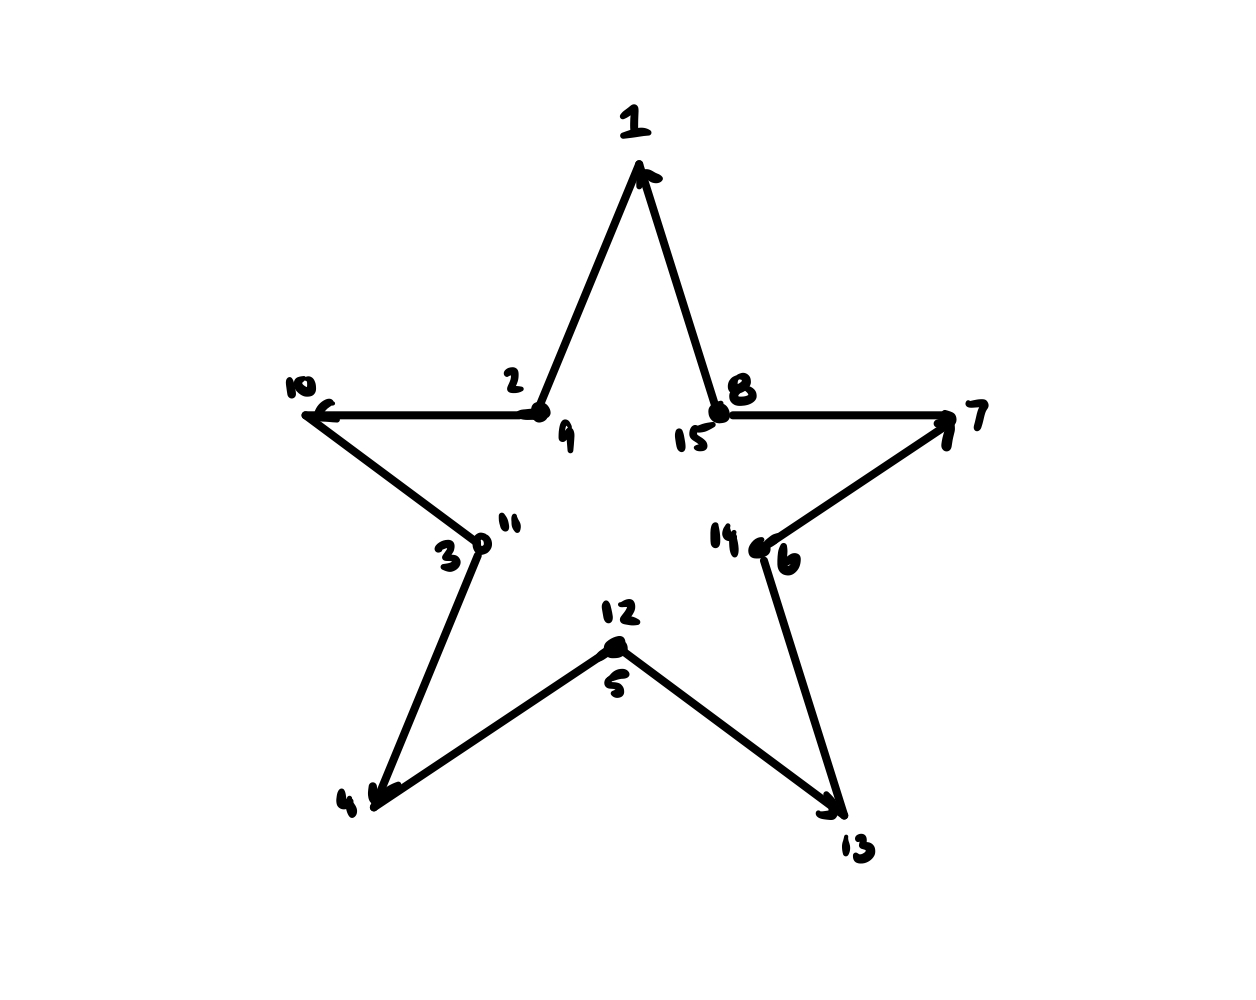
\includegraphics[width=0.8\textwidth]{laser_path.png}
    \caption{Laser Path and Point Order}
    \label{fig:laser_path}
\end{figure}

\end{document}